\documentclass[11pt]{article}
\usepackage[margin=1in]{geometry}
\usepackage{amsmath,amssymb}
\usepackage{booktabs}
\usepackage{graphicx}
\usepackage{hyperref}
\usepackage{natbib}
\usepackage{enumitem}

\graphicspath{{figures/}}

\title{\texttt{stats\_v\_process.ipynb} --- Notebook Documentation}
\author{SLR Forecasting Project}
\date{March 2026}

\begin{document}
\maketitle

\section{Purpose}

This notebook compares the forecasting skill of three approaches to projecting global mean sea level rise (GMSLR):
\begin{enumerate}[noitemsep]
    \item A \textbf{Bayesian rate-and-state semi-empirical model} (``DOLS'') that relates GMSLR rate to global mean surface temperature (GMST) via a quadratic polynomial with a thermal disequilibrium state variable;
    \item \textbf{IPCC AR6 process-model projections}, comprising seven workflows built on ISMIP6 ice-sheet models, glacier models, and thermosteric components;
    \item The \textbf{Vermeer \& Rahmstorf (2009)} dual semi-empirical model (``VR09''), $dH/dt = a(T - T_0) + b\,dT/dt$, included as a second semi-empirical benchmark.
\end{enumerate}
The comparison is carried out using out-of-sample verification against NASA satellite altimetry (2006--2024), hindcast cross-validation with truncated calibration records, and several forecast-horizon diagnostics.

\section{Notebook Structure}

The notebook contains 30 cells organized into 8 sections.

\subsection{Section 1: Data Loading and Baseline Alignment (Cells 1--3)}

All datasets are loaded from the project HDF5 store and rebased so that the year 2000 corresponds to zero sea level and zero temperature anomaly.

\paragraph{Datasets loaded:}
\begin{itemize}[noitemsep]
    \item Frederikse et al.\ tide-gauge GMSL reconstruction (1900--2018, annual, meters)
    \item Berkeley Earth GMST (1850--2024, annual, with 10-year and 20-year Lowess smoothing)
    \item NASA satellite altimetry GMSL (1993--2024, monthly)
    \item IPCC AR6 GMSL projections for SSP1-2.6, SSP2-4.5, SSP3-7.0, SSP5-8.5 (medium confidence, quantile summaries)
    \item IPCC AR6 GMST projections for matching SSPs
\end{itemize}

\paragraph{Baseline alignment:}
IPCC temperatures are shifted from their pre-industrial baseline to the Berkeley Earth 1995--2005 baseline by matching the overlap at 2015.  GMSL is rebased to year 2000 = 0 for all sources.

\subsection{Section 2: Bayesian Rate-and-State Model (Cells 4--6)}

The calibrated Bayesian rate-and-state model is loaded from \texttt{bayesian\_ratestate\_results.json}.  The model expresses the GMSLR rate as
\begin{equation}
    \frac{dH}{dt} = \frac{d\alpha}{dT}\,T^2 + \alpha_0\,T + c + d\,(S - T),
    \label{eq:rate}
\end{equation}
where $T$ is GMST (Berkeley Earth 1995--2005 baseline), $c$ is a background trend, and $S(t)$ is a slow thermal state variable governed by
\begin{equation}
    \tau\,\frac{dS}{dt} = T - S,
    \label{eq:state}
\end{equation}
with relaxation timescale $\tau$.  The term $d\,(S - T)$ represents thermal disequilibrium between fast surface warming and slow deep-ocean/ice-sheet adjustment.

\paragraph{Calibrated coefficients:}
\begin{center}
\begin{tabular}{lrl}
\toprule
Parameter & Value & Unit \\
\midrule
$d\alpha/dT$ & 4.625 & mm\,yr$^{-1}$\,$^\circ$C$^{-2}$ \\
$\alpha_0$   & 5.171 & mm\,yr$^{-1}$\,$^\circ$C$^{-1}$ \\
$c$ (trend)  & 2.632 & mm\,yr$^{-1}$ \\
$d$ (diseq.) & 0.532 & mm\,yr$^{-1}$\,$^\circ$C$^{-1}$ \\
$\tau$       & 18.2  & yr \\
$R^2$        & 0.635 & --- \\
\bottomrule
\end{tabular}
\end{center}

Ensemble projections are generated via Monte Carlo sampling ($N = 2000$) from the joint posterior over $\{d\alpha/dT,\,\alpha_0,\,c,\,d,\,\tau\}$, with temperature scenarios constructed by merging historical Berkeley Earth observations with IPCC SSP projections (shifted to the calibration baseline).

\subsection{Section 3: Quadratic Extrapolation of Observations (Cell 8)}

As a purely kinematic benchmark, GMSL is extrapolated forward using the rate and acceleration estimated at the end of the Frederikse record via a 30-year bandwidth local polynomial:
\begin{equation}
    H(t) = H_{\mathrm{end}} + \dot{H}_{\mathrm{end}}\,(t - t_{\mathrm{end}}) + \tfrac{1}{2}\,\ddot{H}_{\mathrm{end}}\,(t - t_{\mathrm{end}})^2.
\end{equation}
At $t_{\mathrm{end}} \approx 2003$: rate $= 2.98 \pm 0.10$\,mm\,yr$^{-1}$, acceleration $= 0.105 \pm 0.018$\,mm\,yr$^{-2}$.  A separate extrapolation from mid-record NASA satellite GMSL (anchor $\approx 2009$) gives rate $= 3.31$\,mm\,yr$^{-1}$, acceleration $= 0.075$\,mm\,yr$^{-2}$.

Uncertainty is propagated by bootstrap resampling of rate and acceleration from their Gaussian uncertainties ($10^5$ draws).

\subsection{Section 4: Observed Time Series (Cell 10)}

\textbf{Figure 1} shows Frederikse GMSL (cm, left axis) and 10-year smoothed Berkeley Earth GMST ($^\circ$C, right axis) on a common timeline, both rebased to year 2000.

\begin{figure}[htbp]
\centering
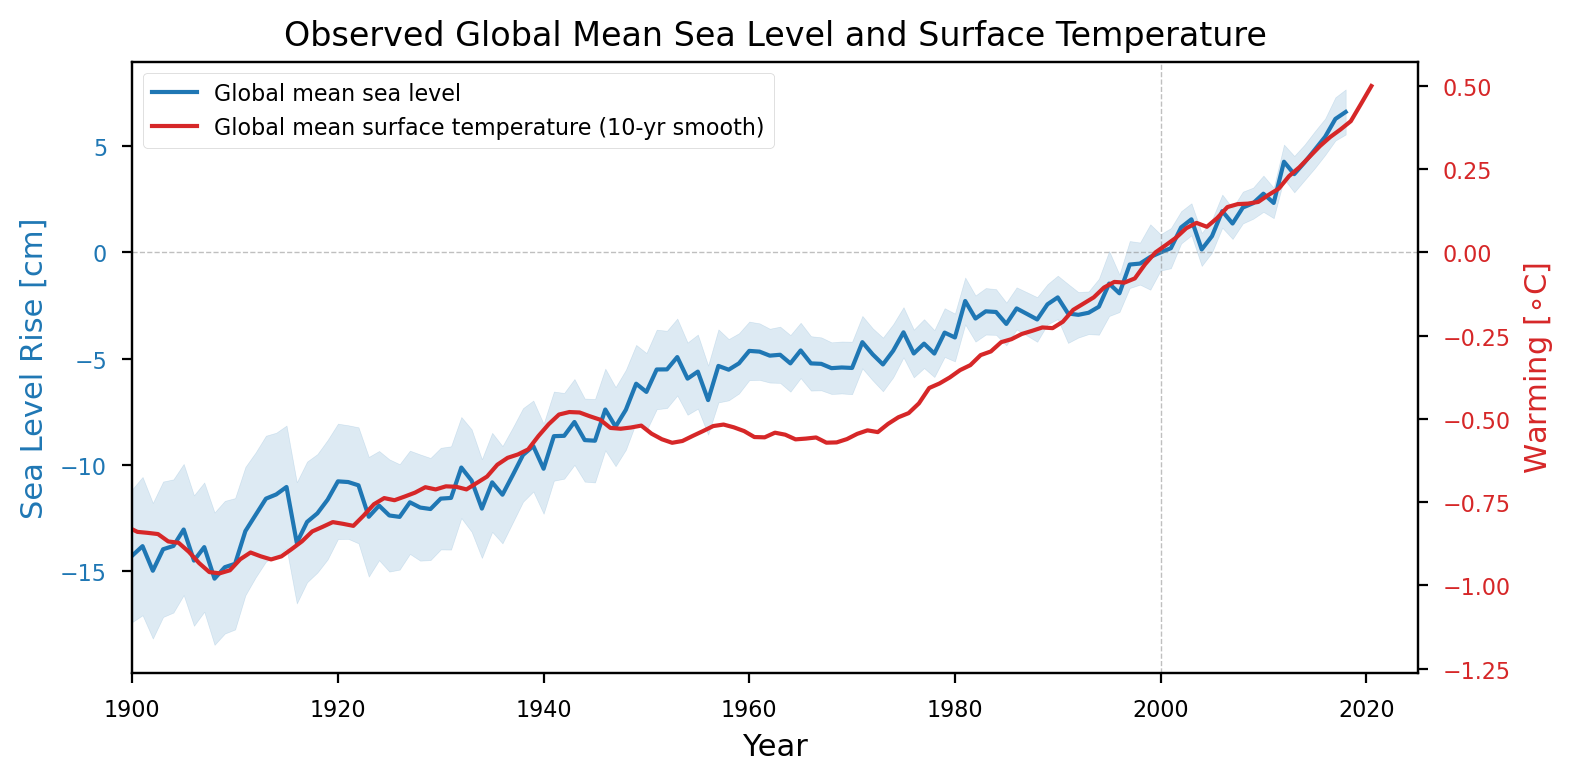
\includegraphics[width=\textwidth]{stats_v_process_fig1_observations.png}
\caption{Observed global mean sea level (Frederikse et al., blue, left axis) and global mean surface temperature (Berkeley Earth 10-year Lowess smooth, red, right axis), both rebased to year 2000. The co-evolution of GMSL and GMST motivates the semi-empirical modelling approach.}
\label{fig:observations}
\end{figure}

\subsection{Section 5: Two-Panel Projection Plot (Cell 12)}

\textbf{Figure 2} is a two-panel figure:
\begin{itemize}[noitemsep]
    \item \textbf{Upper panel:} GMSL projections for SSP2-4.5 from all three sources (observations + kinematic extrapolation, semi-empirical model, IPCC AR6) with 90\% confidence intervals and right-axis societal impact scales (people at risk from Kulp \& Strauss 2019; annual flood costs from Jevrejeva et al.\ 2018).
    \item \textbf{Lower panel:} Observed and projected GMST for the same SSP.
\end{itemize}

\begin{figure}[htbp]
\centering
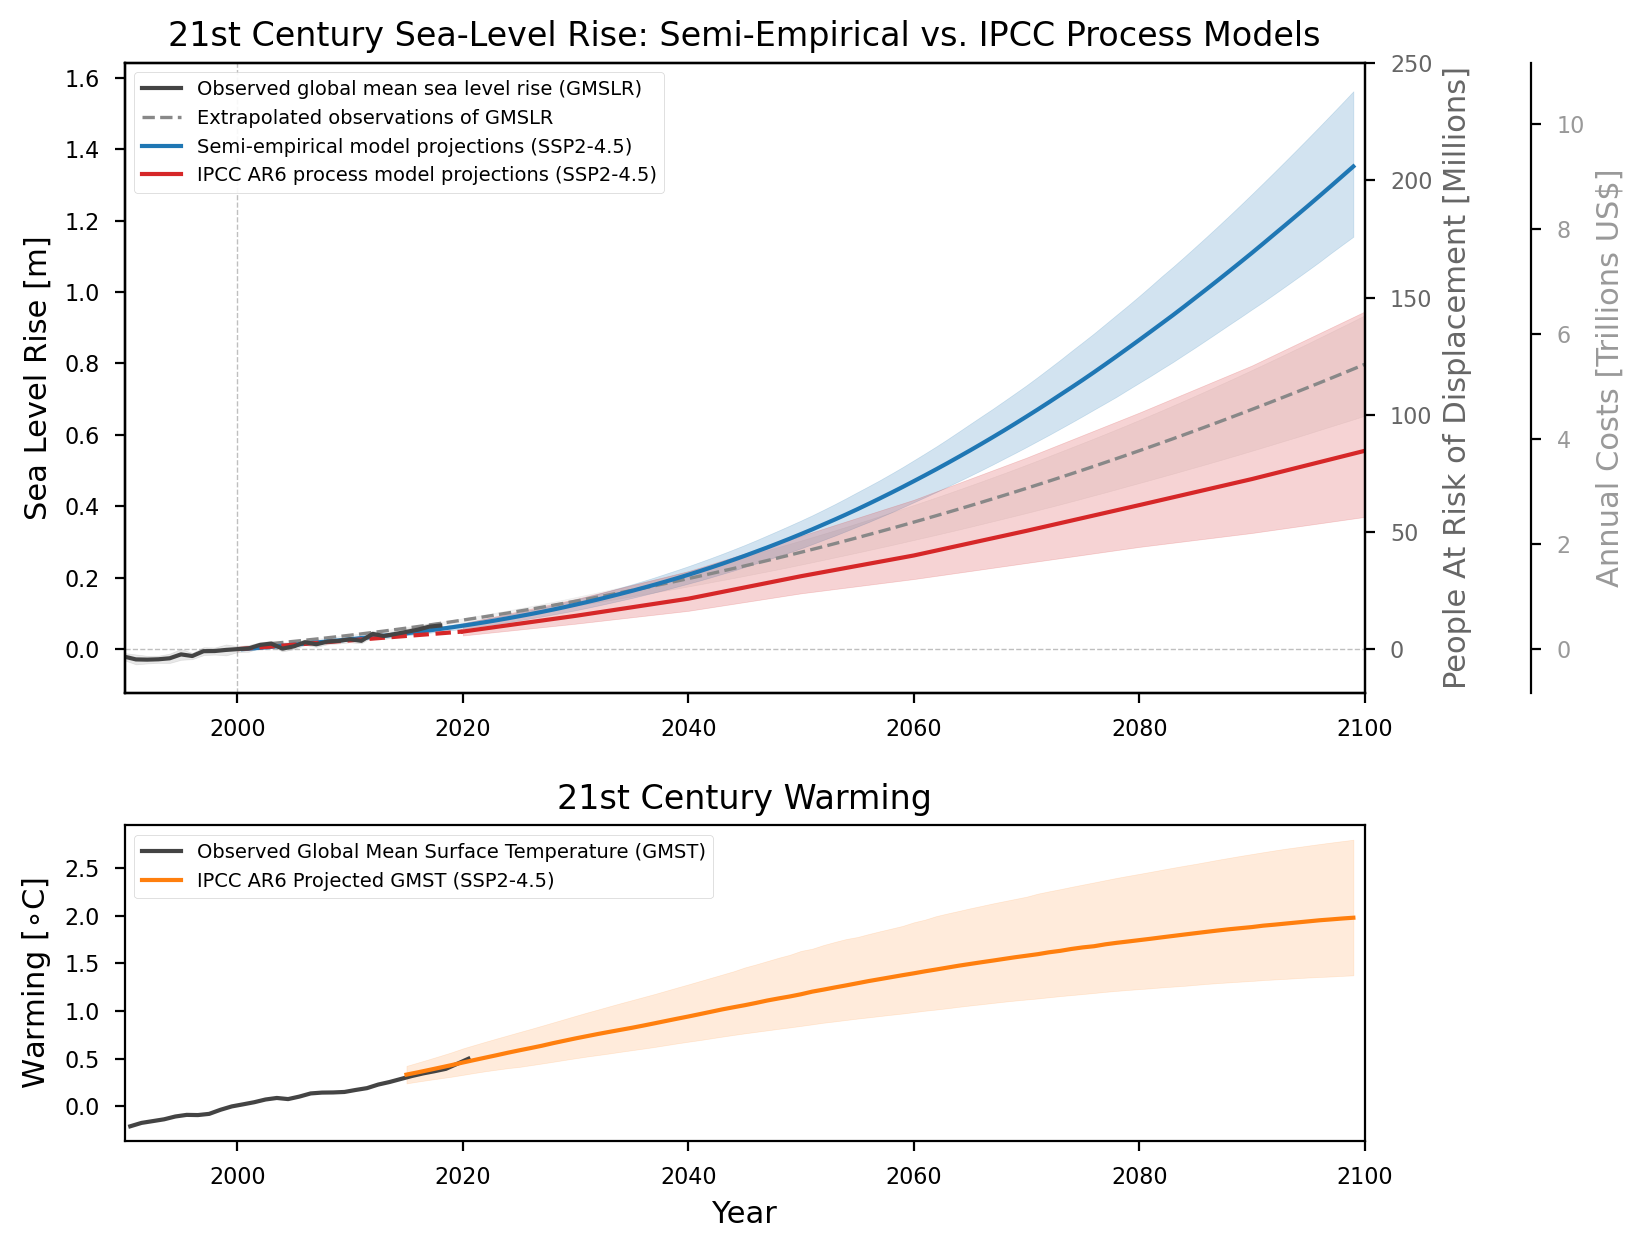
\includegraphics[width=\textwidth]{stats_v_process_fig2_projections.png}
\caption{21st-century projections under SSP2-4.5. \textbf{Upper:} GMSL from observations (dark grey), kinematic extrapolation (dashed grey), semi-empirical rate-and-state model (blue), and IPCC AR6 process models (red), with 90\% confidence intervals. Right axes show people at risk of displacement (Kulp \& Strauss, 2019) and annual flood costs (Jevrejeva et al., 2018). \textbf{Lower:} Observed and projected GMST for the same scenario.}
\label{fig:projections}
\end{figure}

\subsection{Section 6: Hindcast Cross-Validation (Cells 14--18)}

The Bayesian model is re-calibrated on truncated observational records ending at cutoff years 2000, 2010, and 2018.  For each cutoff, the model projects forward using observed Berkeley Earth temperatures merged with SSP2-4.5.

\textbf{Figure 3} shows the hindcast projections with 90\% CIs overlaid on the full Frederikse record.

\begin{figure}[htbp]
\centering
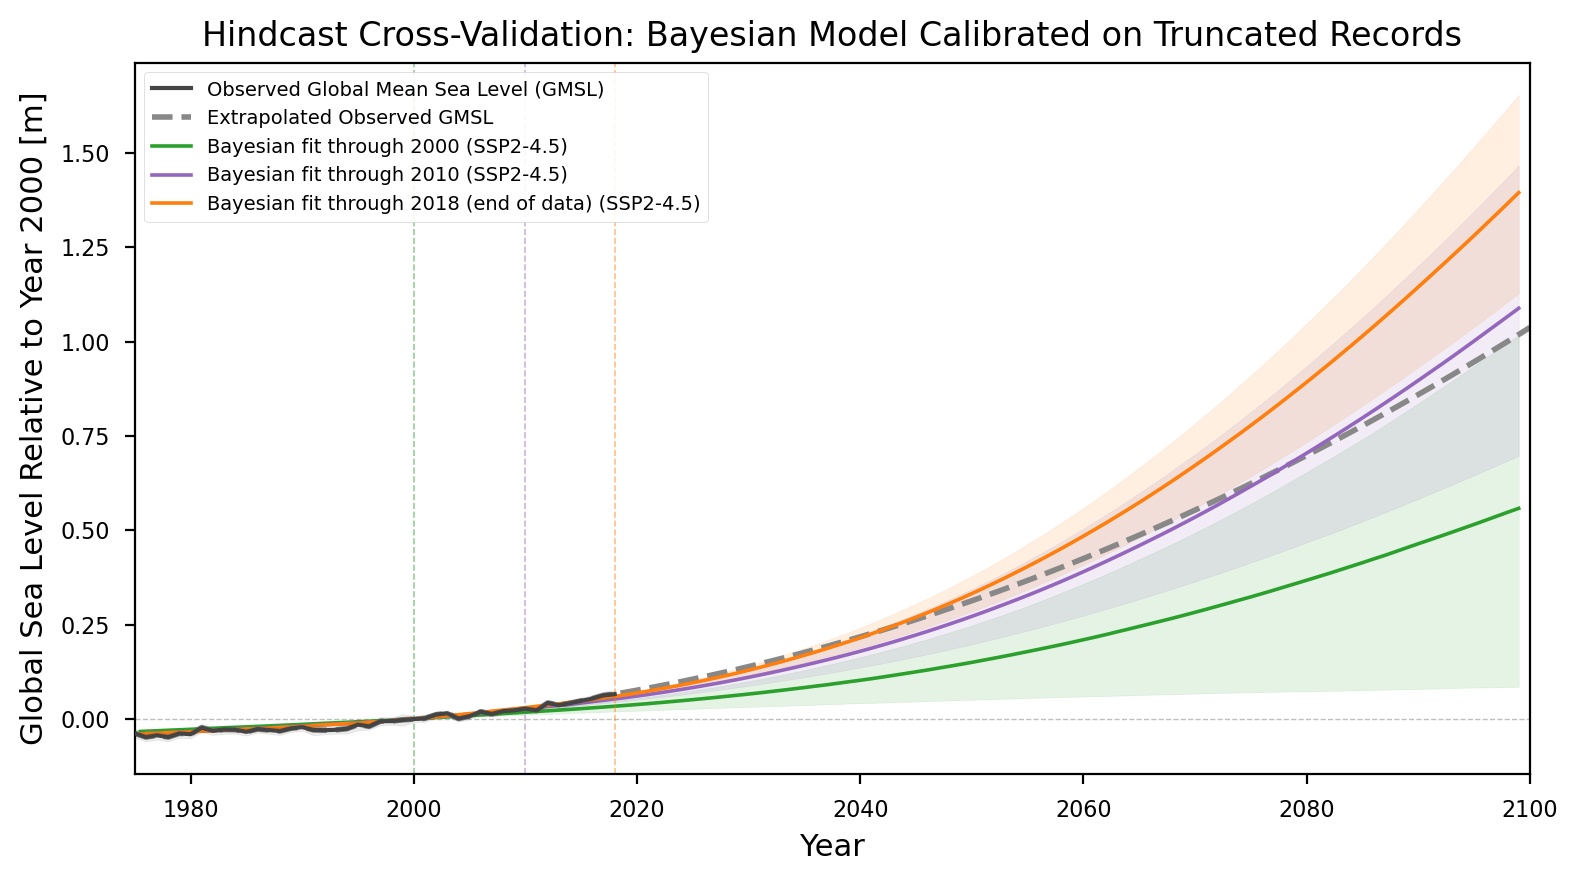
\includegraphics[width=\textwidth]{stats_v_process_fig3_hindcast.png}
\caption{Hindcast cross-validation. The Bayesian rate-and-state model is calibrated on truncated Frederikse GMSL records ending at 2000 (green), 2010 (purple), and 2018 (orange), then projected forward using observed + SSP2-4.5 temperature. Shaded regions show 90\% confidence intervals. The kinematic extrapolation (dashed grey) is shown for comparison. Shorter calibration records produce wider uncertainty and larger bias.}
\label{fig:hindcast}
\end{figure}

\textbf{Figure 4} adds the IPCC AR6 workflow ensembles (7 workflows, each with 20{,}000 MC samples) to the hindcast comparison.

\begin{figure}[htbp]
\centering
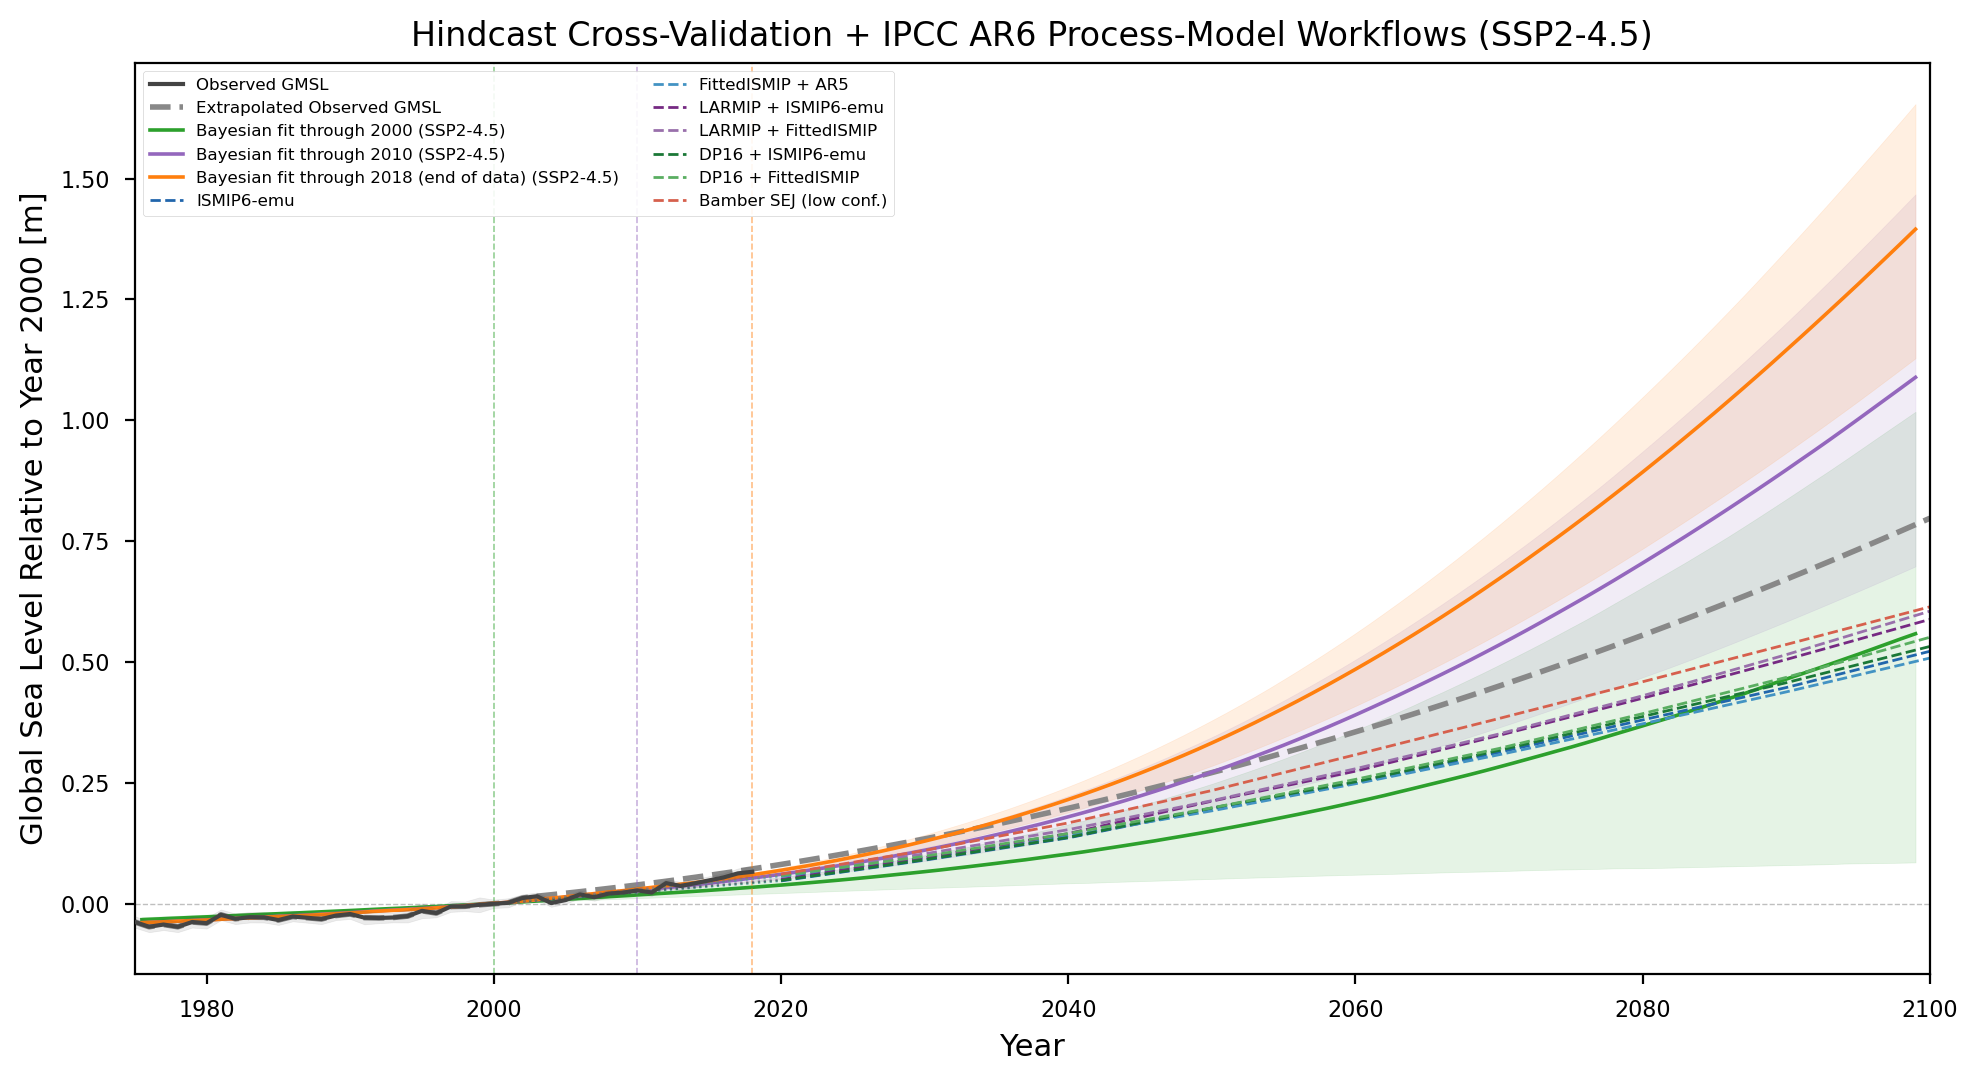
\includegraphics[width=\textwidth]{stats_v_process_fig4_hindcast_ismip6.png}
\caption{Hindcast cross-validation with IPCC AR6 workflow ensembles overlaid. Seven IPCC workflows (colour-coded) are shown alongside the semi-empirical hindcasts from Figure~\ref{fig:hindcast}. IPCC workflow medians at 2100 (SSP2-4.5) range from 508\,mm (wf\_1f) to 614\,mm (wf\_4, Bamber SEJ, low confidence).}
\label{fig:hindcast_ismip6}
\end{figure}

\textbf{Figure 5} compares NASA satellite GMSL, Frederikse tide-gauge GMSL, a mid-record kinematic extrapolation, and all 7 IPCC AR6 workflows.

\begin{figure}[htbp]
\centering
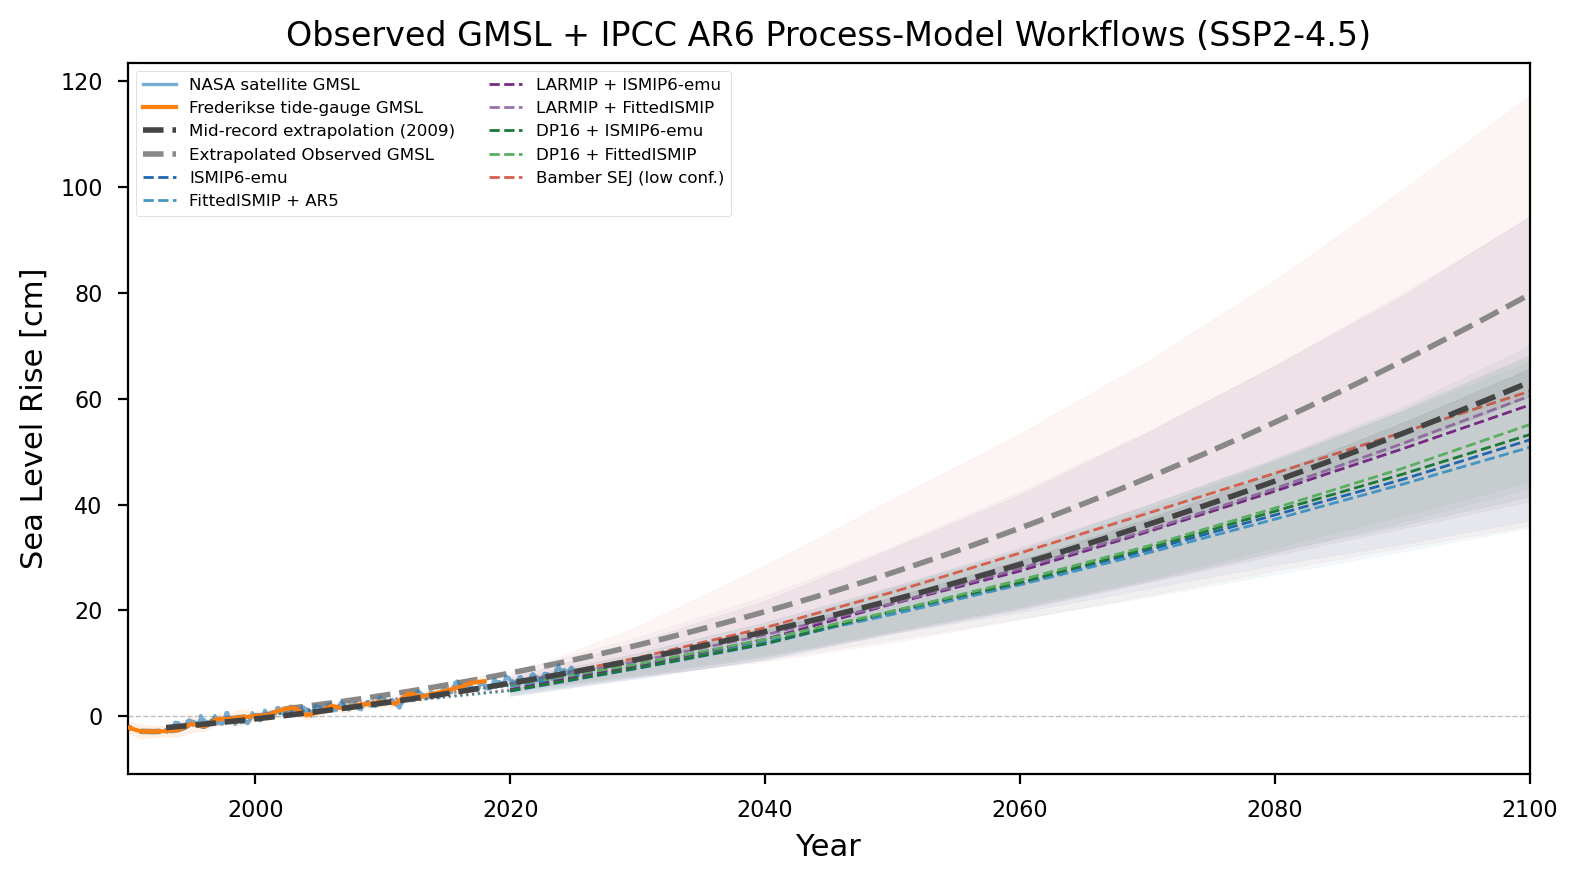
\includegraphics[width=\textwidth]{stats_v_process_fig5_gmsl_observations_ipccar6members.png}
\caption{Observed GMSL from NASA satellite altimetry and Frederikse tide-gauge reconstruction, with mid-record kinematic extrapolation from the satellite era and IPCC AR6 workflow ensemble projections. This figure highlights the relationship between observational trends and the spread of process-model projections.}
\label{fig:obs_ipccar6}
\end{figure}

\paragraph{Hindcast metrics (vs.\ Frederikse, 90\% CI):}
\begin{center}
\begin{tabular}{lccc}
\toprule
Cutoff & RMSE (mm) & Bias (mm) & 90\% Coverage \\
\midrule
2000 & 14.8 & +10.7 & 22\% \\
2010 &  8.6 &  +5.7 & 38\% \\
2018 & --- (end of data) & --- & --- \\
\bottomrule
\end{tabular}
\end{center}

\paragraph{Projection comparison at 2100 (SSP2-4.5):}
\begin{center}
\begin{tabular}{lcc}
\toprule
Source & Median (mm) & 90\% CI (mm) \\
\midrule
Rate-and-state & 1351 & 1155--1562 \\
IPCC AR6       &  555 &  370--945  \\
Difference     & +796 & --- \\
\bottomrule
\end{tabular}
\end{center}

\subsection{Section 7: Forecasting Skill Analysis (Cells 20--24)}

This section performs a rigorous out-of-sample verification of all three model families against NASA satellite altimetry over 2006--2024, using three complementary diagnostics.

\subsubsection{Vermeer \& Rahmstorf (2009) Implementation (Cell 21)}

The VR09 dual model is:
\begin{equation}
    \frac{dH}{dt} = a\,(T - T_0) + b\,\frac{dT}{dt},
\end{equation}
with published parameters $a = 5.6 \pm 0.5$\,mm\,yr$^{-1}$\,K$^{-1}$, $b = -49 \pm 10$\,mm\,K$^{-1}$.  The equilibrium temperature $T_0$ is baseline-dependent; two approaches are tested:
\begin{itemize}[noitemsep]
    \item \textbf{Approach A} (analytical baseline shift): $T_0 = -0.959$\,K.  RMSE $= 35.2$\,mm, bias $= -24.6$\,mm.
    \item \textbf{Approach B} (empirical $T_0$ calibration with $a$, $b$ fixed): $T_0 = -0.864$\,K.  RMSE $= 21.2$\,mm, bias $= -3.1$\,mm.
\end{itemize}
Approach B is adopted. An MC ensemble ($N = 2000$) samples jointly over $(a, b, T_0)$ uncertainties.

\subsubsection{Direct Out-of-Sample Verification (Cell 22)}

\textbf{Figure 6} compares all models against NASA satellite GMSL (2006--2024).

\begin{figure}[htbp]
\centering
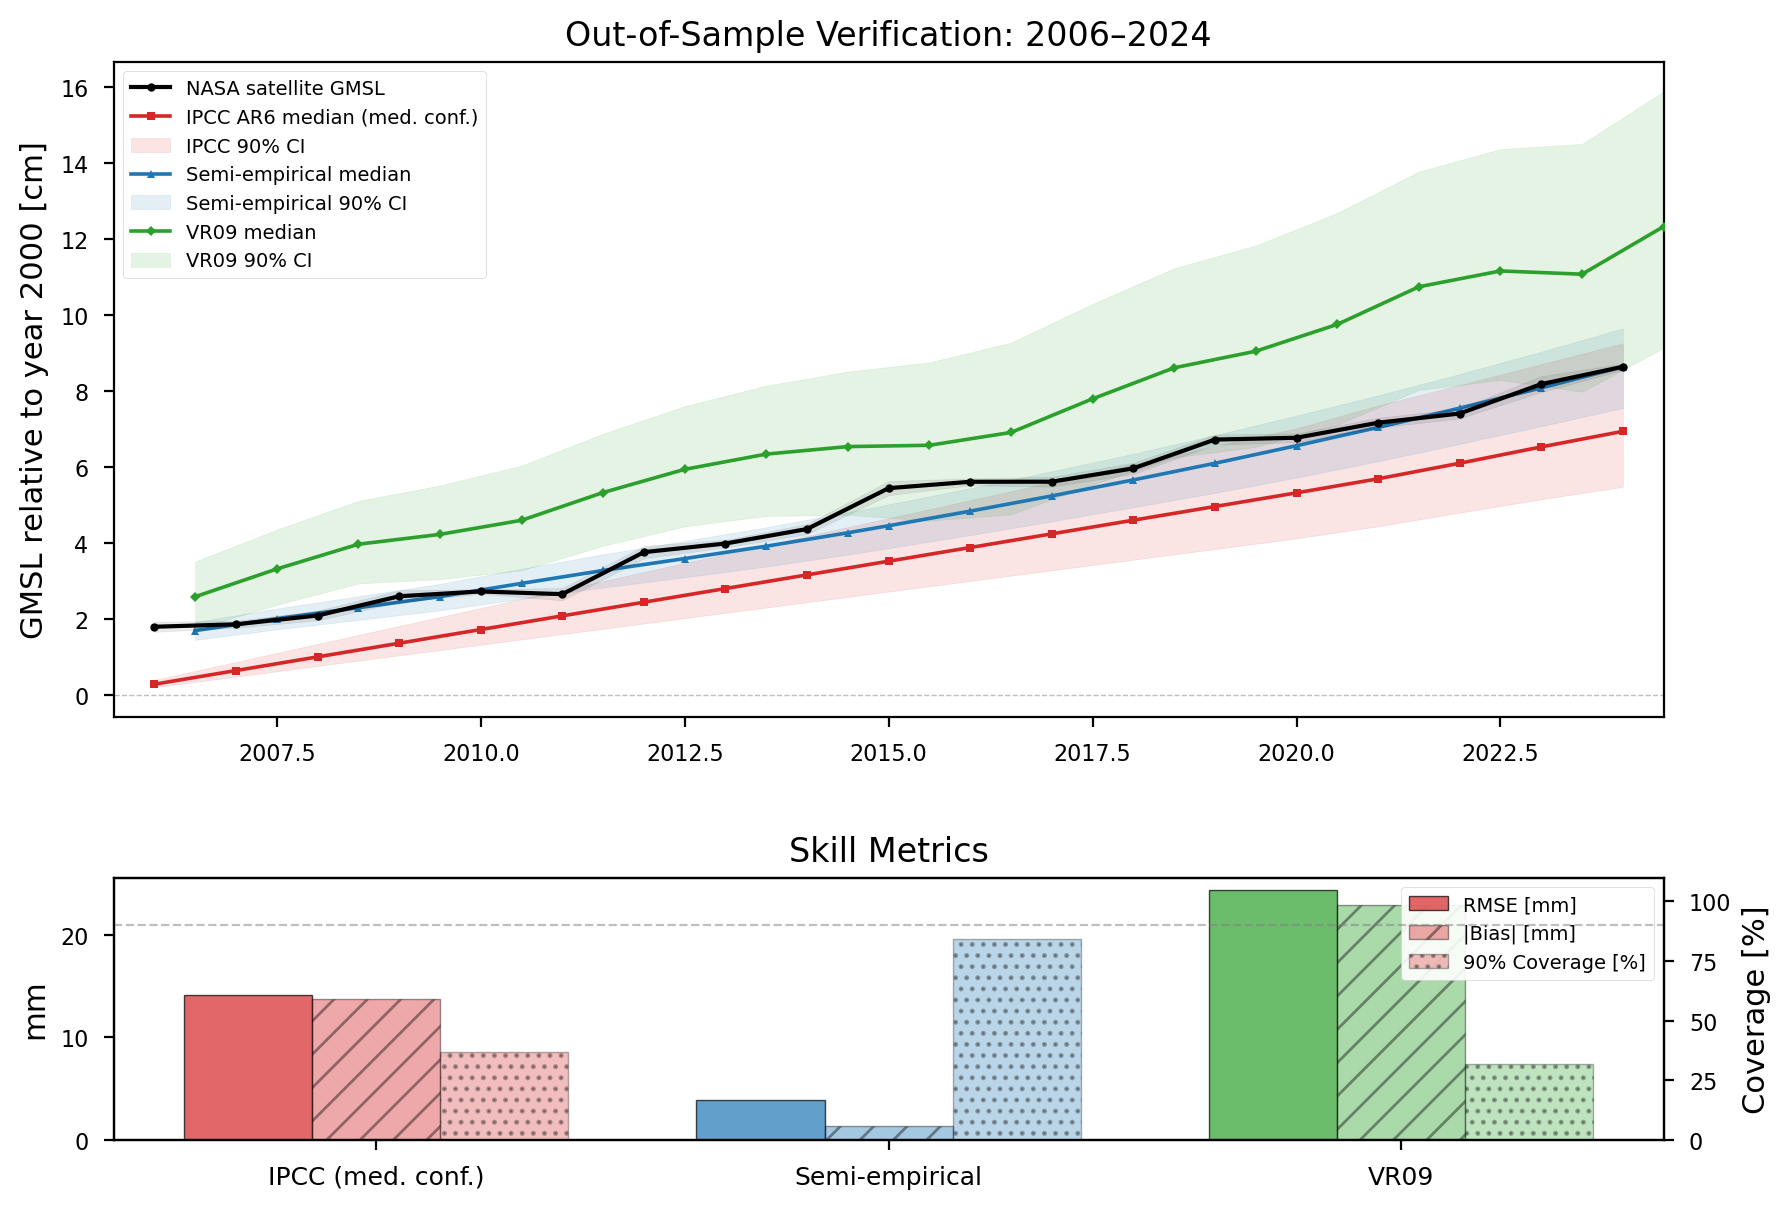
\includegraphics[width=\textwidth]{stats_v_process_fig6_verification.png}
\caption{Direct out-of-sample verification against NASA satellite GMSL (2006--2024). \textbf{Upper:} Time series comparison of observed GMSL (black) with the semi-empirical model (blue), IPCC AR6 combined medium-confidence ensemble (red), and VR09 (green), each with 90\% confidence intervals. \textbf{Lower:} Bar chart of RMSE, bias, and 90\% CI coverage for all IPCC workflows, the semi-empirical model, and VR09. The semi-empirical model achieves the lowest RMSE (3.9\,mm) and highest coverage (84\%).}
\label{fig:verification}
\end{figure}

\begin{center}
\begin{tabular}{lccc}
\toprule
Model & RMSE (mm) & Bias (mm) & 90\% Coverage \\
\midrule
Semi-empirical (DOLS) &  3.87 & +1.37 & 84\% \\
IPCC combined (med.\ conf.) & 14.07 & +13.73 & 37\% \\
VR09 & 24.35 & $-$22.90 & 32\% \\
\midrule
\multicolumn{4}{l}{\textit{Individual IPCC workflows:}} \\
Bamber SEJ (wf\_4, low conf.) & 8.74 & +8.13 & 63\% \\
LARMIP + FittedISMIP (wf\_2f) & 10.08 & +9.69 & 74\% \\
ISMIP6-emu (wf\_1e) & 17.82 & +17.32 & 0\% \\
\bottomrule
\end{tabular}
\end{center}

The DOLS model has the lowest RMSE, smallest bias, and highest CI coverage among all models tested.  IPCC workflows systematically overpredict early-period GMSL (positive bias), while VR09 strongly underpredicts (negative bias).

\subsubsection{Reliability Analysis (Cell 23)}

\textbf{Figure 7} presents probability integral transform (PIT) histograms and reliability (coverage) diagrams for the three model families.

\begin{figure}[htbp]
\centering
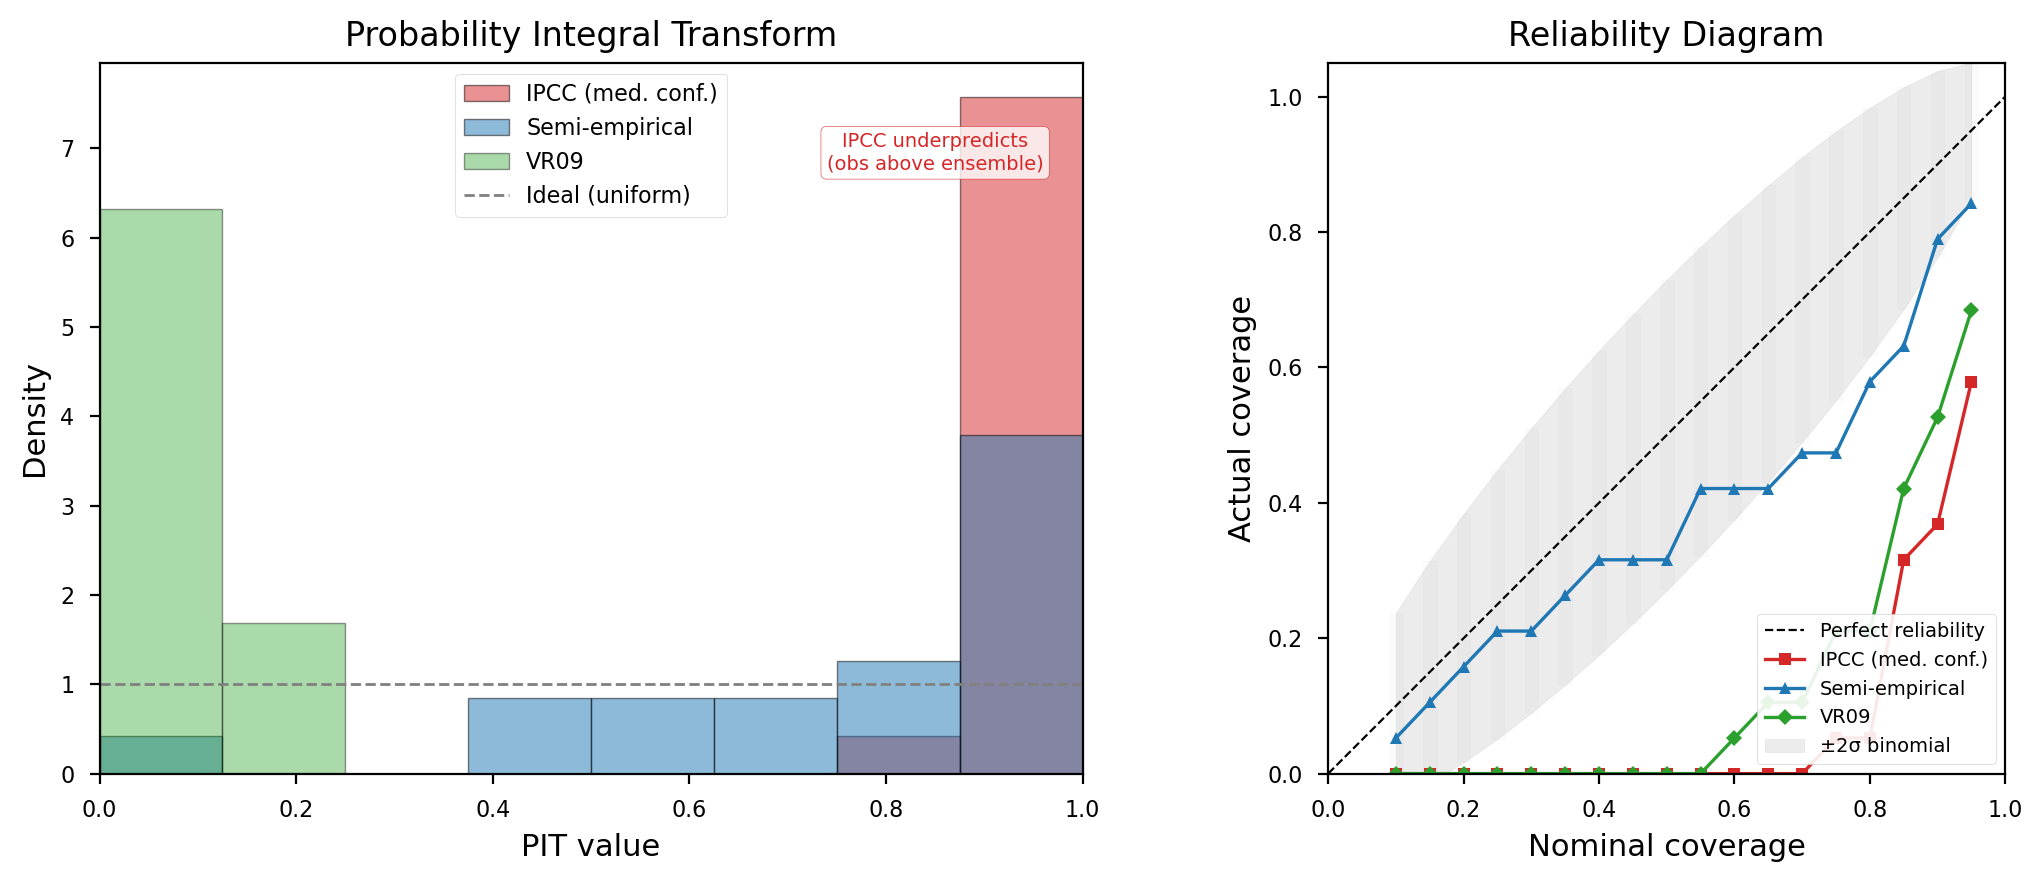
\includegraphics[width=\textwidth]{stats_v_process_fig7_reliability.png}
\caption{Reliability analysis. \textbf{Left:} PIT histograms for the IPCC combined ensemble, the semi-empirical model (DOLS), and VR09. A well-calibrated model produces a uniform histogram. The IPCC histogram is concentrated near 1.0 (systematic underprediction of observed GMSL); VR09 is concentrated near 0.0 (systematic overprediction); DOLS is closest to uniform but skewed toward high values. \textbf{Right:} Reliability (coverage) diagrams showing actual vs.\ nominal coverage at each confidence level. The diagonal represents a perfectly calibrated model.}
\label{fig:reliability}
\end{figure}

The PIT is the CDF value at which the observation falls within each model's ensemble distribution at each verification year.  A well-calibrated model produces PIT values uniformly distributed on $[0, 1]$.

\begin{center}
\begin{tabular}{lcccc}
\toprule
Model & PIT Mean & KS Statistic & $p$-value & 90\% Coverage \\
\midrule
IPCC  & 0.956 & 0.875 & $< 0.001$ & 37\% \\
DOLS  & 0.762 & 0.412 & 0.002     & 79\% \\
VR09  & 0.072 & 0.778 & $< 0.001$ & 53\% \\
\bottomrule
\end{tabular}
\end{center}

All models fail the KS uniformity test, but the DOLS model is closest to calibrated (PIT mean $= 0.762$ vs.\ the ideal $0.50$).  The IPCC PIT mean near 1.0 confirms systematic underprediction; VR09's near-zero PIT mean confirms systematic overprediction.

\subsubsection{Conditional Skill Analysis (Cell 24)}

\textbf{Figure 8} investigates whether skill differences arise from temperature forcing uncertainty or from the GMSL model itself.  The DOLS model is re-evaluated using observed Berkeley Earth GMST only (no SSP switch at end of record), isolating the sea-level model's skill from temperature scenario uncertainty.

\begin{figure}[htbp]
\centering
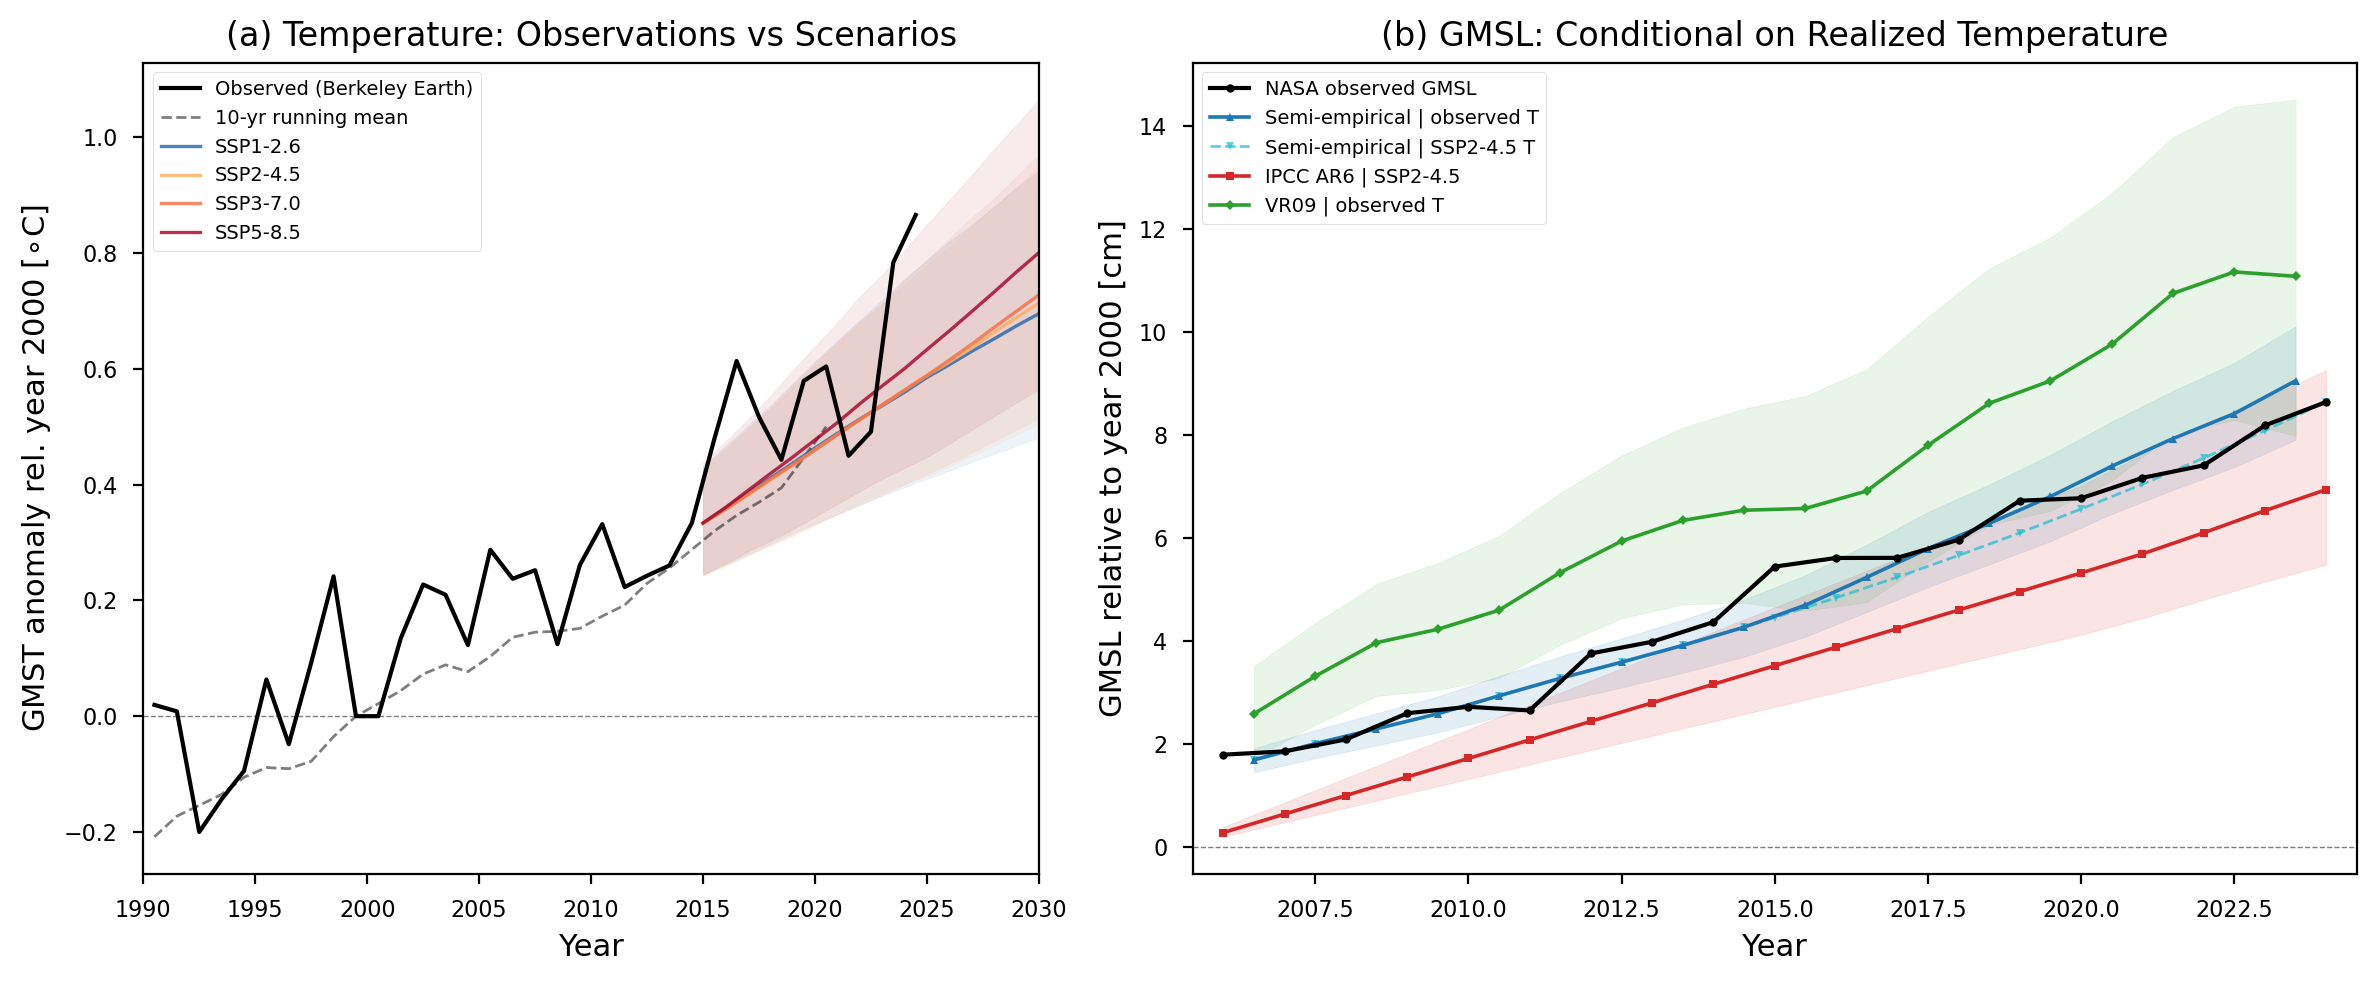
\includegraphics[width=\textwidth]{stats_v_process_fig8_conditional.png}
\caption{Conditional skill analysis. \textbf{Left:} Observed GMST (Berkeley Earth) and SSP2-4.5 projected temperature over the verification period, showing that realized warming closely tracks the SSP2-4.5 scenario through 2024. \textbf{Right:} GMSL projections conditioned on observed temperature only (no SSP switch), with 90\% CIs. The DOLS model conditioned on observed temperature achieves RMSE~$= 5.5$\,mm and 89\% coverage, confirming that its skill derives from the sea-level model rather than temperature scenario accuracy.}
\label{fig:conditional}
\end{figure}

\begin{center}
\begin{tabular}{lccc}
\toprule
Configuration & RMSE (mm) & Bias (mm) & 90\% Coverage \\
\midrule
DOLS $|$ observed $T$ &  5.46 & $-$2.47 & 89\% \\
DOLS $|$ SSP2-4.5 $T$ &  3.87 & +1.37  & --- \\
IPCC $|$ SSP2-4.5     & 14.07 & +13.73 & 37\% \\
VR09 $|$ observed $T$  & 23.62 & $-$22.35 & 37\% \\
\bottomrule
\end{tabular}
\end{center}

When conditioned on observed temperature, the DOLS model achieves RMSE $= 5.5$\,mm with 89\% coverage at the 90\% nominal level.  The IPCC bias is not attributable to temperature forcing because SSP2-4.5 closely tracks observed warming through 2024.

\subsection{Section 8: Forecast Horizon Analysis (Cells 26--28)}

Three diagnostics assess how model skill degrades with lead time and extrapolation beyond the calibration domain.

\subsubsection{Hindcast Degradation Curves (Cell 26)}

\textbf{Figure 9} re-calibrates both DOLS and VR09 for cutoff years from 1960 to 2010 (in 10-year steps), projects forward with observed temperature only, and bins RMSE and 90\% CI coverage by 5-year lead time.

\begin{figure}[htbp]
\centering
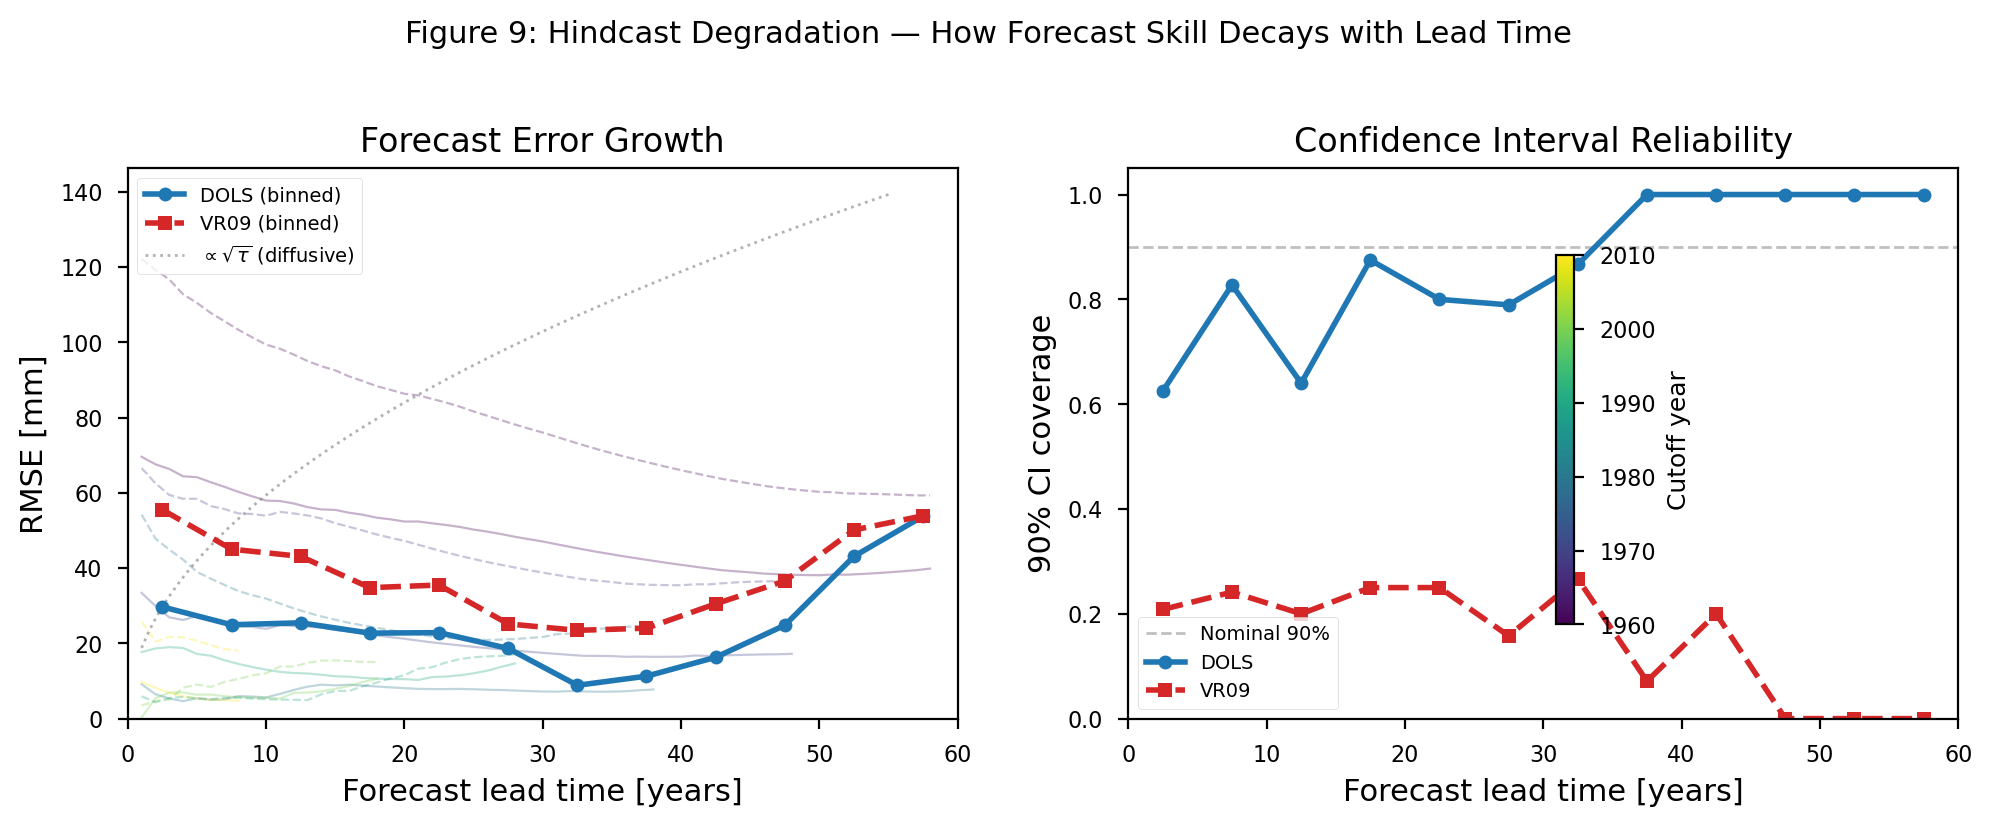
\includegraphics[width=\textwidth]{stats_v_process_fig9_degradation.png}
\caption{Hindcast degradation curves. RMSE (left) and 90\% CI coverage (right) as a function of forecast lead time for the semi-empirical model (DOLS, blue) and VR09 (green), computed by re-calibrating on records truncated at 1960--2010 and verifying against subsequent observations. DOLS error remains below $\sim$27\,mm at all leads and coverage stays at or above 62\%. VR09 error grows steadily and coverage falls to 0\% at leads exceeding 35 years.}
\label{fig:degradation}
\end{figure}

Key findings:
\begin{itemize}[noitemsep]
    \item DOLS RMSE remains below $\sim$27\,mm at all lead times up to 58 years and \emph{decreases} at longer leads (most recent data has highest information content).  Coverage stays at or above 62\%, reaching 100\% at leads $> 35$\,years.
    \item VR09 RMSE grows to $\sim$54\,mm at 58-year lead and coverage falls to 0\%.
\end{itemize}

\subsubsection{Temperature Exceedance Analysis (Cell 27)}

\textbf{Figure 10} quantifies how far projected temperatures exceed the maximum observed during calibration.

\begin{figure}[htbp]
\centering
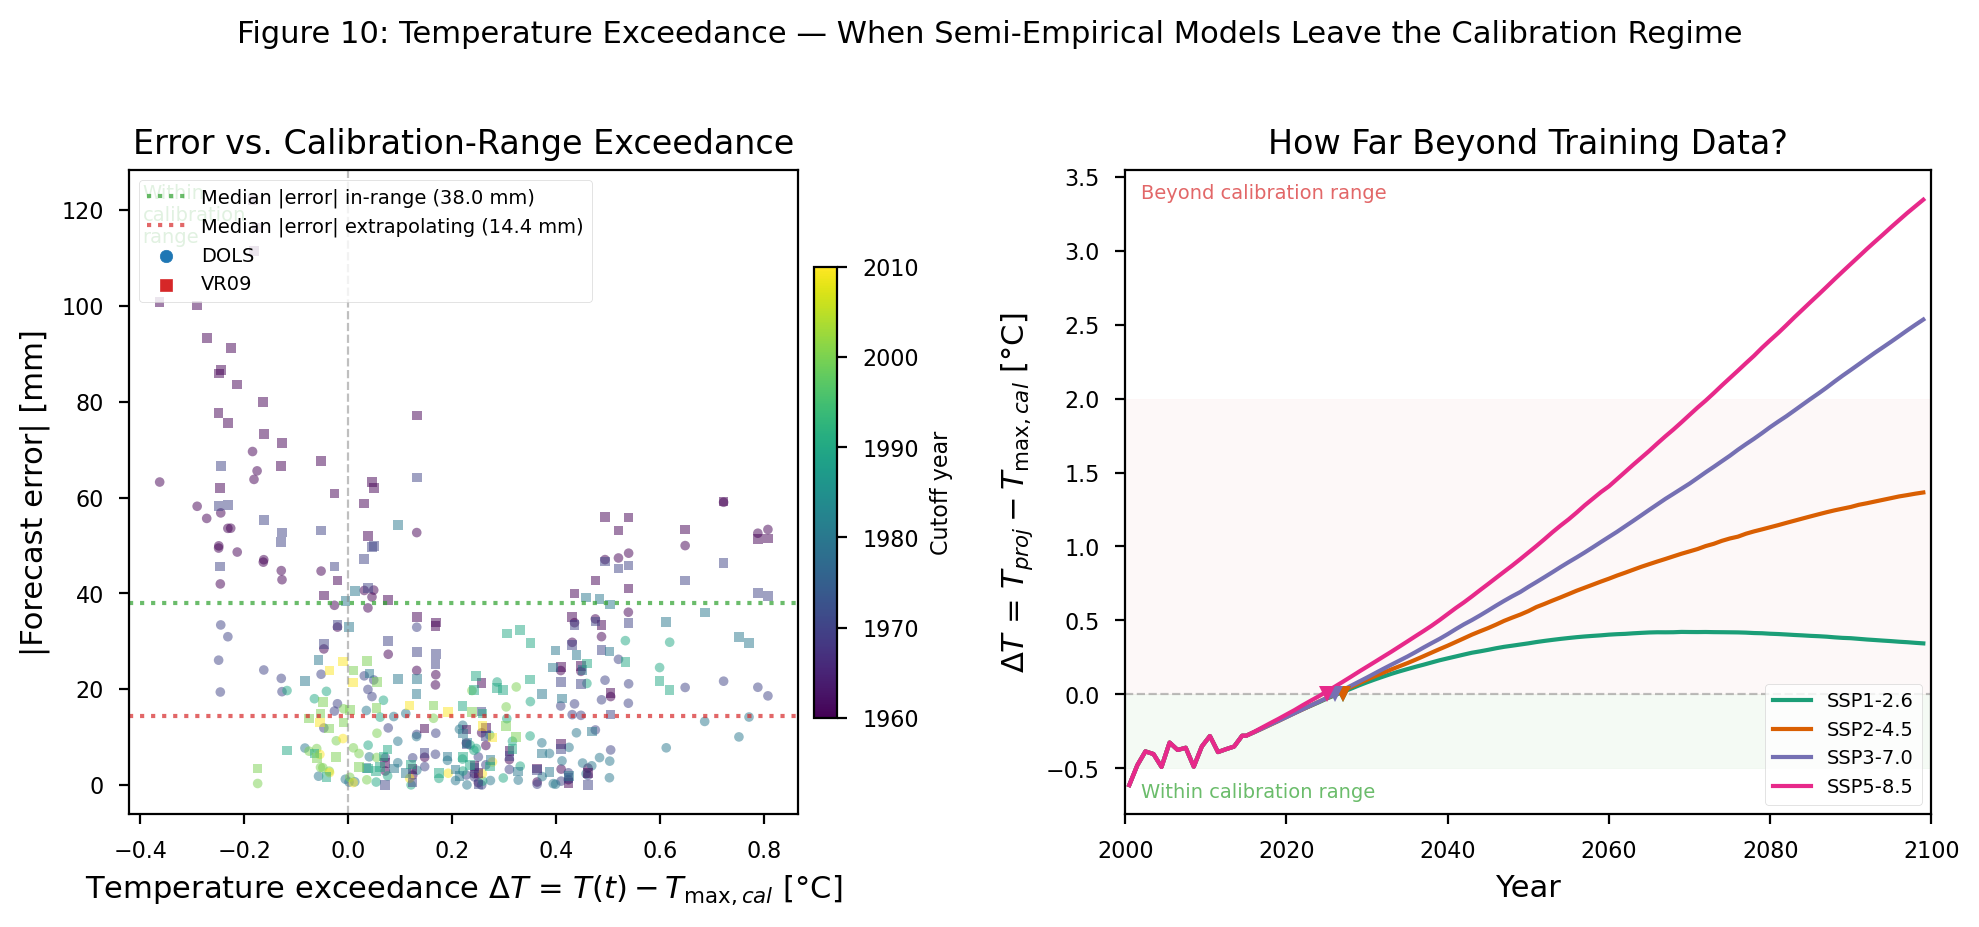
\includegraphics[width=\textwidth]{stats_v_process_fig10_exceedance.png}
\caption{Temperature exceedance analysis. Projected GMST under each SSP relative to the maximum temperature in the calibration record ($T_{\max} = 0.49\,^\circ$C, Berkeley Earth 1995--2005 baseline). All SSPs enter the extrapolation regime ($T > T_{\max}$) around 2025--2027. The semi-empirical model's absolute error is plotted against temperature exceedance, showing that errors in the extrapolation regime are not systematically larger than errors within the calibration range.}
\label{fig:exceedance}
\end{figure}

The full calibration record (1920--2018) has $T_{\max} = 0.492\,^\circ$C (Berkeley Earth 1995--2005 baseline).  All SSPs enter the temperature extrapolation regime around 2025--2027:
\begin{center}
\begin{tabular}{lcc}
\toprule
SSP & Exceedance Year & $\Delta T$ at 2100 ($^\circ$C) \\
\midrule
SSP1-2.6 & 2027 & +0.34 \\
SSP2-4.5 & 2027 & +1.36 \\
SSP3-7.0 & 2026 & +2.53 \\
SSP5-8.5 & 2025 & +3.34 \\
\bottomrule
\end{tabular}
\end{center}

Counterintuitively, the median absolute error is \emph{smaller} in the extrapolation regime (11.6\,mm, $n = 298$) than within the calibration range (31.2\,mm, $n = 98$), likely because recent (warmer) data is most informative for near-future projections.

\subsubsection{Cross-Model Divergence (Cell 28)}

\textbf{Figure 11} compares DOLS, VR09, kinematic extrapolation, and IPCC AR6 on a common grid (2000--2100, SSP2-4.5).  The inter-model standard deviation ($\sigma_{\mathrm{inter}}$) is compared to the mean intra-model uncertainty ($\sigma_{\mathrm{intra}}$).

\begin{figure}[htbp]
\centering
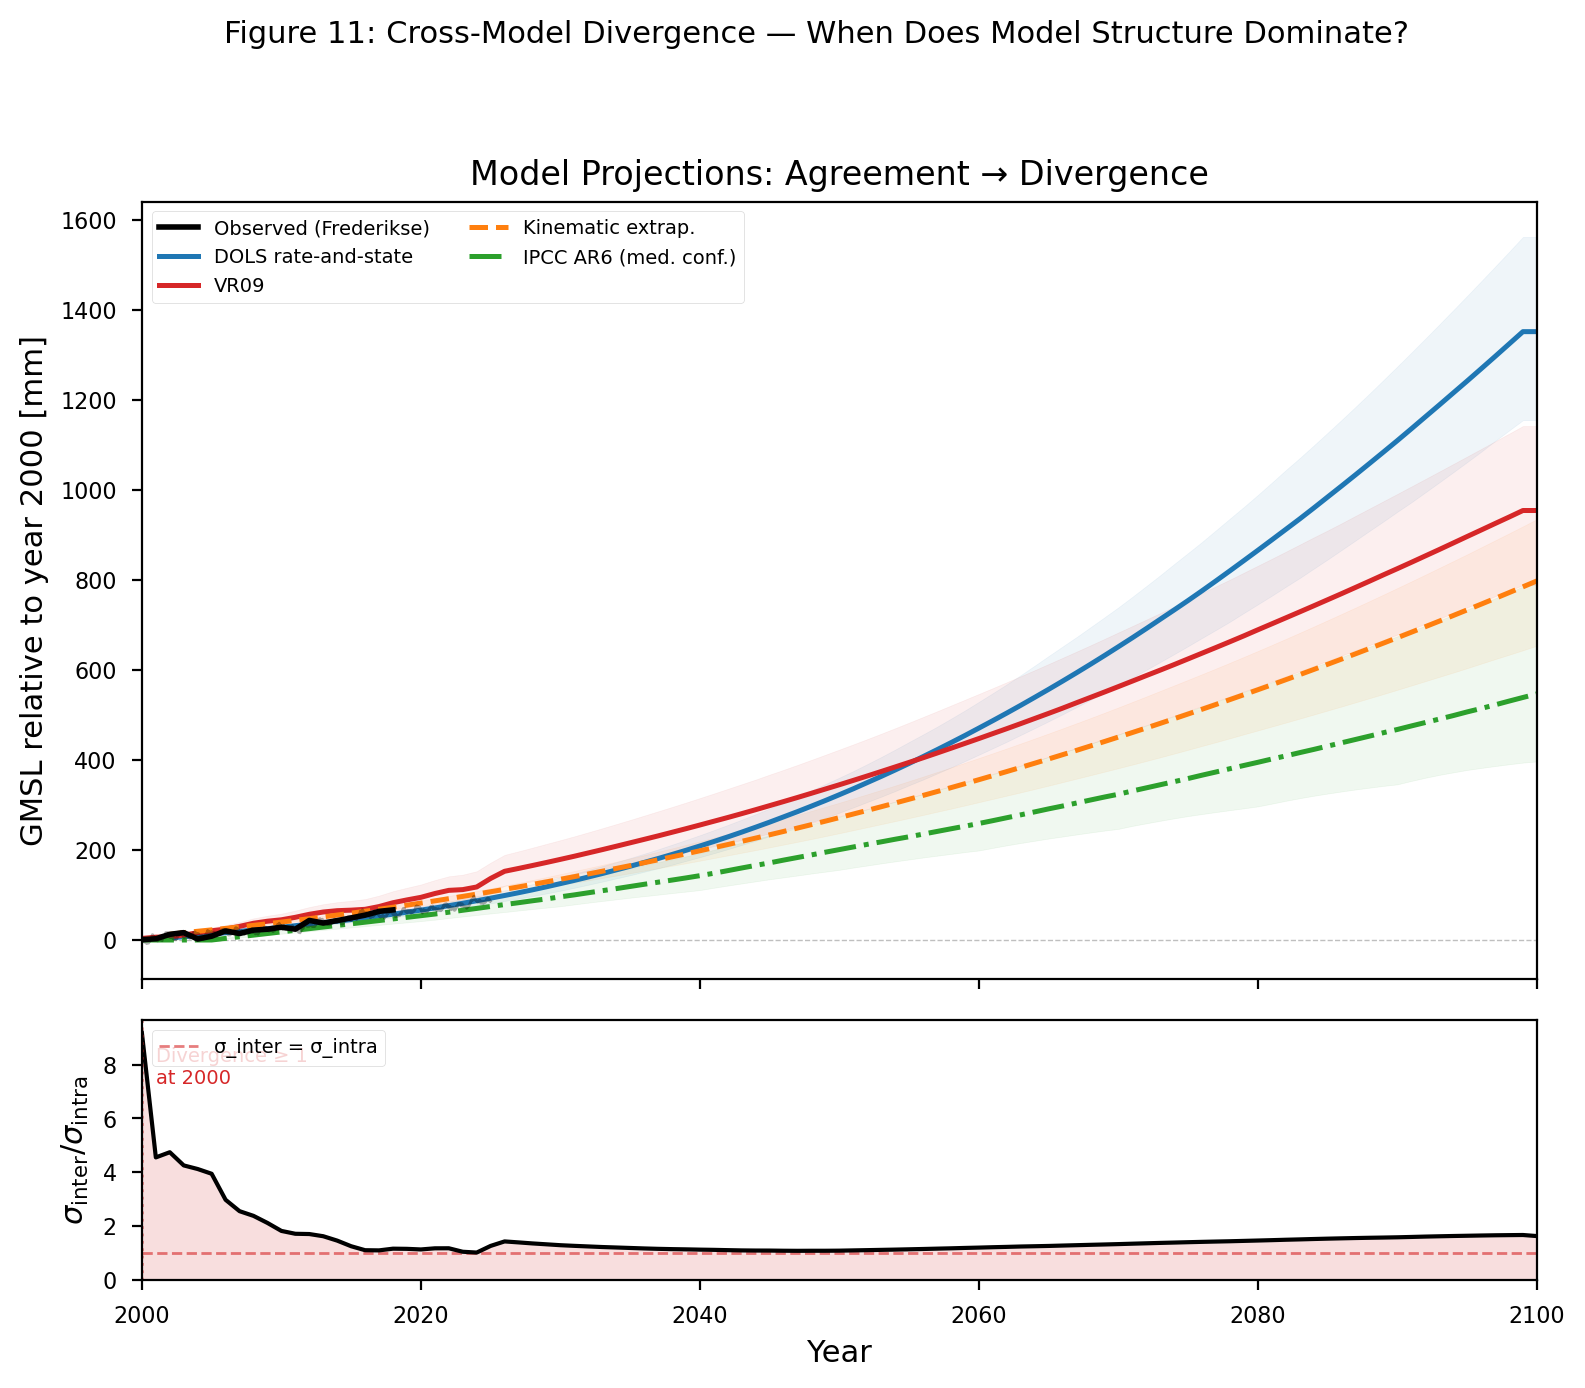
\includegraphics[width=\textwidth]{stats_v_process_fig11_divergence.png}
\caption{Cross-model divergence under SSP2-4.5. \textbf{Upper:} GMSL projections from the semi-empirical model (DOLS), VR09, kinematic extrapolation, and IPCC AR6, each with 90\% confidence intervals. \textbf{Lower:} Ratio of inter-model standard deviation ($\sigma_{\mathrm{inter}}$) to mean intra-model uncertainty ($\sigma_{\mathrm{intra}}$). A ratio exceeding 1.0 indicates that structural model differences dominate over parametric uncertainty within any single model. The ratio is $\geq 1$ at all projection times and reaches 1.62 at 2100.}
\label{fig:divergence}
\end{figure}

\begin{center}
\begin{tabular}{lcccccc}
\toprule
Year & DOLS & VR09 & Kinematic & IPCC & $\sigma_{\mathrm{inter}}$ & $\sigma_{\mathrm{inter}}/\sigma_{\mathrm{intra}}$ \\
     & (mm) & (mm) & (mm)      & (mm) & (mm) & \\
\midrule
2030 &  125 &  178 &  134 &   95 &  30 & 1.28 \\
2050 &  322 &  344 &  271 &  200 &  55 & 1.08 \\
2100 & 1351 &  954 &  797 &  546 & 291 & 1.62 \\
\bottomrule
\end{tabular}
\end{center}

The inter-model spread exceeds the intra-model uncertainty at all times ($\sigma_{\mathrm{inter}}/\sigma_{\mathrm{intra}} \geq 1$), indicating that structural model differences dominate over parametric uncertainty.  At 2100, the divergence ratio reaches 1.62.

\section{Key Figures}

\begin{enumerate}
    \item \textbf{Figure 1:} Observed GMSL + GMST twin-axis time series (1900--2024).
    \item \textbf{Figure 2:} Two-panel GMSL/GMST projection with societal impact axes.
    \item \textbf{Figure 3:} Hindcast cross-validation (DOLS at cutoffs 2000, 2010, 2018).
    \item \textbf{Figure 4:} Hindcast cross-validation with IPCC AR6 workflow ensembles overlaid.
    \item \textbf{Figure 5:} NASA satellite GMSL + Frederikse + kinematic extrapolation + IPCC AR6 workflows.
    \item \textbf{Figure 6:} Direct out-of-sample verification (2006--2024) with skill metrics.
    \item \textbf{Figure 7:} PIT histograms and reliability diagrams.
    \item \textbf{Figure 8:} Conditional skill analysis (observed vs.\ SSP temperature).
    \item \textbf{Figure 9:} Hindcast degradation curves (RMSE and coverage vs.\ lead time).
    \item \textbf{Figure 10:} Temperature exceedance analysis.
    \item \textbf{Figure 11:} Cross-model divergence ($\sigma_{\mathrm{inter}}$ vs.\ $\sigma_{\mathrm{intra}}$).
\end{enumerate}

\section{Dependencies}

The notebook imports from the following project modules:
\begin{itemize}[noitemsep]
    \item \texttt{slr\_analysis.py} --- DOLS calibration (\texttt{calibrate\_dols}), kinematics (\texttt{compute\_kinematics}), resampling
    \item \texttt{slr\_data\_readers.py} --- societal impact functions (\texttt{people\_displaced\_kulpstrauss2019}, \texttt{slr\_cost\_jevrejeva2018})
    \item \texttt{slr\_projections.py} --- MC ensemble projections (\texttt{project\_gmsl\_state\_ensemble})
    \item \texttt{bayesian\_dols.py} --- ODE solver and Bayesian fitting (\texttt{solve\_state\_ode}, \texttt{fit\_bayesian\_level})
    \item \texttt{slr\_ar6\_member\_readers.py} --- IPCC AR6 full-sample component readers (224 NetCDF files, 7 workflows)
\end{itemize}

Data are stored in \texttt{data/processed/slr\_processed\_data.h5} (53 keys) and \texttt{data/raw/ipcc\_ar6/} (FACTS NetCDF files).

\section{Reproducibility}

\begin{itemize}[noitemsep]
    \item All random number generators use explicit seeds (42, 99, etc.) for reproducibility.
    \item Monte Carlo ensemble size: $N = 2{,}000$ (DOLS, VR09); $N = 20{,}000$ per workflow (IPCC); $N = 120{,}000$ combined medium-confidence.
    \item Verification window: NASA satellite GMSL, 2006--2024 (19 annual values).
    \item IPCC workflows interpolated from decadal to annual resolution for year-by-year comparison.
\end{itemize}

\end{document}
